%%%%%%%%%%%%%%%%%% DOCUMENT SETUP %%%%%%%%%%%%%%%%%%

% Required IEEE parameters
%\documentclass[letterpaper, 10pt, conference]{llncs} % set document type
\documentclass[runningheads]{llncs}
%\IEEEoverridecommandlockouts                              % for \thanks command
%\overrideIEEEmargins                             % use for \addtolength to normalize column lengths


% Packages
\usepackage{graphicx} % allows additional graphics formats
  \graphicspath{ {./images/} }
\usepackage{amsmath}   % assumes amsmath package installed
  \allowdisplaybreaks[1] % allow eqnarrays to break across pages
\usepackage{amssymb}   % assumes amsmath package installed 
\usepackage{url}       % format hyperlinks correctly
\usepackage{rotating}  % allow portrait figures and tables
\usepackage{subfigure} % allow matrices of figures
\usepackage{float}     % allows H option on floats to force here placement
\usepackage{multirow}  % allows merging of rows in tables
\usepackage{tabularx}  % allows fixed width tables
\usepackage{ctable}    % modifies \hline for use in table
\usepackage{bm}        % allow bold fonts in equations
\usepackage{wrapfig}   % allow text wrapping round figures
\usepackage{stfloats}  % control placement of floats
\usepackage[backend=biber,style=ieee,maxbibnames=3,bibencoding=utf8]{biblatex}   % allow bibliography control 
  \addbibresource{journal_abbreviations.bib}
  \addbibresource{references.bib}
\usepackage{siunitx}
\usepackage{placeins}
\usepackage[ruled,vlined]{algorithm2e}
\include{pythonlisting}
% Custom commands
\newcommand{\matlab}{\emph{\sc{Matlab}}}
\newcommand{\maple}{\emph{\sc{Maple}}}
\newcommand{\simulink}{\emph{\sc{Simulink}}}
\newcommand{\dc}{d.c.}
\newcommand{\ac}{a.c.}
\newcommand{\rms}{RMS}
\newcommand{\wgn}{{\tt wgn}}
\newcommand{\sus}[1]{$^{\mbox{\scriptsize #1}}$}
\newcommand{\sub}[1]{$_{\mbox{\scriptsize #1}}$}
\newcommand{\chap}[1]{Chapter~\ref{#1}}
\newcommand{\sect}[1]{Section~\ref{#1}}
\newcommand{\fig}[1]{Fig.~\ref{#1}}
\newcommand{\tab}[1]{Table~\ref{#1}}
\newcommand{\equ}[1]{(\ref{#1})}
\newcommand{\appx}[1]{Appendix~\ref{#1}}
\newcommand{\degree}{\ensuremath{^\circ}}
\newcommand{\Vrms}{V\sub{\rms}}
\newcommand{\Vpp}{V\sub{pp}}
\newcommand{\otoprule}{\midrule[\heavyrulewidth]}         
\newcolumntype{Z}{>{\centering\arraybackslash}X}  % tabularx centered columns 
\newcommand\norm[1]{\left\lVert#1\right\rVert}

%\usepackage{setspace}


\usepackage{flushend}
% Adjust figure spacing to get more text onto each page
\setlength{\abovecaptionskip}{2pt}
\setlength{\belowcaptionskip}{2pt}
\setlength{\dbltextfloatsep}{8pt}
\setlength{\dblfloatsep}{3pt}
\setlength{\floatsep}{3pt}
\setlength{\textfloatsep}{2pt}
%\addtolength{\skip\footins}{-10pt}


%%%%%%%%%%%%%%%%%% TITLE AND FRONT MATTER %%%%%%%%%%%%%%%%%%
\begin{document}

\thispagestyle{empty} % stop page numbers
\pagestyle{empty}

\title{Intrusion detection and classification with autoencoded deep neural network}
%
%\titlerunning{Abbreviated paper title}
% If the paper title is too long for the running head, you can set
% an abbreviated paper title here
%
\author{Shahadate Rezvy\inst{1}\orcidID{0000-0002-2684-7117}, Miltos Petridis\inst{1}\orcidID{0000-0003-1275-1023}, Aboubaker Lasebae \inst{1}\orcidID{0000-0003-2312-9694}, \and
Tahmina Zebin \inst{2}\orcidID{0000-0003-0437-0570} }
%
\authorrunning{F. Author et al.}
% First names are abbreviated in the running head.
% If there are more than two authors, 'et al.' is used.
%
\institute{Middlesex University , London, United Kingdom \\
\email{\{s.rezvy, M.Petridis, A.Lasebae\}@mdx.ac.uk}\\
 \and
University of Manchester, United Kingdom\\
\email{\{tahmina.zebin\}@manchester.ac.uk}}
%
\maketitle              % typeset the header of the contribution
%
\begin{abstract}
A Network Intrusion Detection System  is a critical component of every internet connected system due to likely attacks from both external and internal sources. A NIDS is used to detect network born attacks such as denial of service attacks, malware, and intruders that are operating within the system. Neural networks have become an increasingly popular
solution for network intrusion detection. Their capability of learning complex patterns and behaviors make them a suitable solution for differentiating between normal traffic and network attacks. In this paper, we have applied a deep autoencoded dense neural network algorithm for detecting intrusion or attacks in network connection and evaluated the algorithm with the benchmark NSL-KDD dataset. Our  results  showed  an  excellent  performance  with  an overall  detection  accuracy  of  99.3\%  for  Probe,  Remote to Local,  Denial of Service and  User to Root type  of attacks. We also presented a comparison with recent approaches used in literature which showed a substantial improvement in terms of accuracy and speed of detection with the proposed algorithm.

\keywords{Deep learning \and secure computing \and intrusion detection system \and autoencoder \and dense neural network.}
\end{abstract}



%%%%%%%%%%%%%%%%%% ABSTRACT %%%%%%%%%%%%%%%%%%





%https://pdfs.semanticscholar.org/39a1/abcbb87d8ff48ee47d446411a3455451f25b.pdf

%%%%%%%%%%%%%%%%%% INTRODUCTION %%%%%%%%%%%%%%%%%%
{\section{Introduction} \label{sec:introduction}}
Over the past few decades, the Internet has penetrated all aspects of our lives. Experts
predict that by 2020 there would be 50 billion connected devices. As technology
becomes more and more integrated, the challenge to keep the systems safe and away
from vulnerability or attacks increases. Over the years we have seen an increase in hacks
in banking systems, healthcare systems and many Internet of Things (IoT) devices \cite{Shone2018}.
These attacks cause billions of dollars in losses every year and loss of systems at crucial times. This has led to higher importance in cyber security specifically in the intrusion detection systems. A related challenge with most modern-day infrastructure is that data requirements pertaining to security are often an afterthought. It is assumed that this impacts the results of any machine learning algorithm applied towards the problem; however, an analysis contrasting the differences are yet to be seen. In addition to this, there is little research in the results of applying next level analysis using deep learning algorithms to determine if there is an improvement in accuracy versus its traditional machine learning counterparts. Deep learning (hierarchical learning) is part of a broader family of machine learning methods based on learning data representations, as opposed to task-specific algorithms. Recently, deep learning
based methods have been successfully implemented in NIDS applications. Deep learning can substitute for manually designed feature extraction to create more secure firewall or intrusion detector \cite{ref:survey18}.

% However, for the practitioner it is difficult to select the most suitable deep learning method for their application. 
 In this work, we have proposed a data mining based hybrid intrusion detection system for distinguishing normal and intrusive events from the NSL-KDD dataset \cite{NSLKDD}.
We focused on exploring low latency models  while  maintaining  high  accuracy  by  proposing a deep auto-encoded dense neural network (DNN) framework for effective intrusion detection. The NIDS using deep learning did alleviate the need of feature selection or feature engineering during the detection process.  In our design, the autoencoder facilitated an unsupervised pre-tarining on the data to provide compressed and less noisy representation of the input space, while the final dense neural network functioned as the supervised classifier for our experimental intrusion detection scenario.


 %rewrite this section once finished

The remainder of this paper is organized as follows. \sect{sec:methods} introduces the background literature in the recent development in intrusion detection systems using deep learning techniques, we then provide details on our parameter settings for the implemented model in section III. The performance of the developed model for attack classification is evaluated in section IV. We also compared the results with some recent deep learning techniques appeared in the literature using the same dataset. Finally, the paper is concluded in section V along with ideas for future work.
\\



%%%%%%%%%%%%%%%%%% BACKGROUND %%%%%%%%%%%%%%%%%%


%%%%%%%%%%%%%%%%%% METHODS %%%%%%%%%%%%%%%%%%

\section{ Background Literature} \label{sec:methods}
%     \begin{figure}
%       \centering
% %       \includegraphics[width=0.45\textwidth]{classifier_architecture.png}
%       \caption{Proposed deep neural network architecture for attack type classification.}
%       \label{fig:architecture}
%     \end{figure}
In recent years, machine learning has been widely applied to problems in detecting network attacks, particularly novel attacks.  Given the landscape of the Internet, machine learning can be applied to handle the massive amounts of traffic to determine what is malicious or benign. NIDS are classifiers that differentiate unauthorized or anomalous
traffic from authorized or normal traffic. \fig{fig:NIDS} shows an illustration of the propoed components for the NIDS implementation. As can be seen in the diagram, the network gateways and routers devices could potentially host an NIDS.
In the recent past, researchers have investigated a wide variety of Machine Learning techniques to design intrusion detection systems for normal and attack classification. However the NIDS design community  suffered from some major challenges as there are very few labeled traffic dataset from real networks for developing an NIDS. Additionally, effective feature selection from the Network Traffic dataset for anomaly detection is difficult. The features selected for one class of attack may not work well for other categories of attacks due to continuously changing and evolving attack scenarios. %It can help optimize the use of resources, whether human or machine. The solution to the bigger picture of cyber security is that different solutions need to exist at every layer of the network to effectively say that a network is "secure." Machine learning is just part of a bigger picture, 
%https://dl.acm.org/citation.cfm?id=2954780

 \begin{figure*}
    \centering
  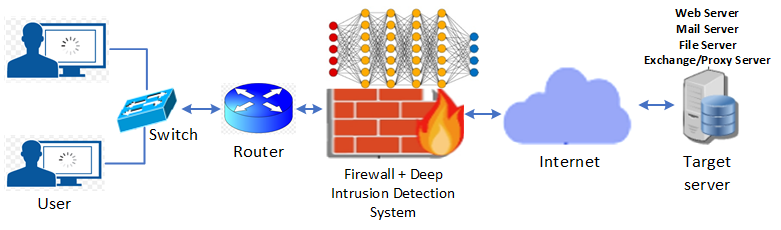
\includegraphics[width=0.85\textwidth]{Figures/NIDS.png}
    \caption{Illustration of the proposed network intrusion detection system(NIDS)}
    \label{fig:NIDS}
  \end{figure*}
  
% https://www.ijcaonline.org/archives/volume180/number14/jayaswal-2018-ijca-916270.pdf


Because of the lack of public data sets for network-based IDSs,  we used the NSL-KDD dataset (which may not be a perfect representation of existing real networks) to compare different intrusion detection methods.
However, traditional machine learning methods depend heavily on feature engineering, and extracting features is often time-consuming and complex. Thus, it is impractical to detect attacks with traditional machine learning methods in real-time applications \cite{LIU2018}. To set our research in context, in the next subsection, we present a literature review on the intrusion detection systems that used deep learning techniques and the NSL-KDD dataset for their performance benchmarking. 
%%%%%%%%%%%%%%%%%%%%%%%%%%%%%%%%%%%%%%%%%%%%%%%%%%%%%%%%%%%%%%%%%%%%  
  \begin{table*}[t]
\centering
\caption{ Attack types in the KDD Cup 1999 dataset \cite{kdd1999} }
\label{table:KDD}
{\def\arraystretch{1.5}\tabcolsep=10pt
\begin{tabular}{p{2cm} p{4cm} p{3cm} }
\toprule
Attack Type 	& Description of the Attack &	Categories 	\\
\otoprule

Denial of Service (DoS)
 & {A DoS attack is a type of attack in which the hacker
makes a computing resources or memory too busy
or too full to serve legitimate networking requests
and hence denying users access to a machine.} &	{apache, back, land, mailbomb, neptune, pod,
processtable, smurf, teardrop, udpstorm.} \\
Probe & {Probing is an attack in which the hacker scans a
machine or a networking device in order to
determine weaknesses or vulnerabilities that may
later be exploited so as to compromise the system.}	& {ipsweep, mscan, nmap, portsweep, saint, satan}\\

Remote to Local (R2L) 
 & {A remote to user attack is an attack in which a user sends packets to a machine over the internet, which
s/he does not have access to in order to expose
the machines vulnerabilities and exploit privileges
which a local user would have on the computer} &	{ftpwrite, guesspassword, imap, multihop, named, phf, sendmail, snmpgetattack, snmpguess, warezmaster, worm, xlock, xsnoop, httptunnel.}\\

User to Root (U2R)  
 & {User to root attacks are exploitations in which the hacker starts off on the system with a normal user
account and attempts to abuse vulnerabilities in the system in order to gain super user privileges.} &	{bufferoverflow, loadmodule, perl, rootkit, ps, sqlattack, xterm.}\\


\bottomrule
\end{tabular}}
\end{table*}




\subsubsection*{Deep machine learning for intrusion detection:}
Neural networks have become an increasingly popular solution for network intrusion detection systems (NIDS). Their capability of learning complex patterns and behaviors make them a suitable solution for differentiating between normal traffic and network attacks \cite{Yisroel2018}. One of the earliest work found in literature that used deep learning approach with Deep Belief Network (DBN) as a feature selector and Support Vector Machine (SVM) as a classifier was reported in \cite{salama2011}. This approach resulted in an accuracy of 92.84\% when applied on training data of NSL-KDD dataset. We observed a use of Artificial neural networks (ANN) with enhanced resilient back-propagation for the design  in ref \cite{Naoum2012} . This work also used the training dataset only by subdividing it in three parts (training (70\%), validation (15\%) and testing (15\%)). The inclusion of the unlabeled data for testing resulted in a reduction of performance for this method. Ref \cite{Pandeeswari2016} applied fuzzy clustering based ANN that resulted above 80\% detection accuracy of with a low false positive rate.  In \cite{Gao2014}, the work used an unsupervised greedy learning algorithm to learn similarity representations over the nonlinear and high-dimensional data in KDD dataset.The results show that four-hidden-layer Restricted Boltzmann machines can produce the higher accuracy in comparison with SVM and ANN.
A deep Neural Network is essentially a multilayer perceptron, which was initially developed by stacking linear classifiers. The model is fed inputs, inputs get multiplied by weights and the passed into an activation function. The model uses backpropagation to adjust weights and increase accuracy. Deep Neural Networks with three or more hidden layers support higher generalization capability in comparison to ANN \cite{Kaynar2017}.
In \cite{Li2015}, a deep belief network for malicious code detection method was reported that included an autoencoder based dimensionality reduction technique. An accelerated
deep architecture was introduced in Potluri et al. \cite{potluri2016} to identify the abnormalities in the network data. They evaluated the performance of the model training related to different processor types and number of cores. Li et al. \cite{Li2017} presented an intrusion detection method using convolutional neural networks which adopts a novel representation learning method of graphic conversion. However, the model accuracy ranged from 79\% to 81.57\% which did not justify the increased latency added by the representation learning of the feature space. In reference \cite{Vinay2017}, Vinaykumar et al. reported various convolutional and recurrent neural network architectures for IDS implementation, however their results for under-represented remote to local (R2L) and user to root (U2R) attacks were very low. Shone et al.\cite{Shone2018} reported a stacked non-symmetric deep auto-encoders with random forest classifier achieved an overall accuracy of 85.42\%, with very poor performance on the R2L and U2R intrusion categories. A stacked autoencoder based implementation of NIDS by Farahnakian et al.  \cite{Farah2018} produced high accuracy (94.71\%) and high detection rate (94.53\%), however, these models could still be improved. 
The findings from our literature review have shown that despite the high detection accuracy being achieved, with most researchers still experimenting
on combining various algorithms (e.g. training, optimisation, activation and classification) and layering approaches to produce the most accurate and efficient solution for a
specific dataset.

In our research, we focused on exploring low latency models while maintaining high accuracy by proposing a hybrid deep neural network that includes an unsupervised pre-training using autoencoders to make the model more adaptive to the changes in the network traffic. We then used a dedicated supervised dense neural network structure for the final classification. In our design, we made sure the memory or processing power to train and execute machine learning models are within the capability of the routers processing power. We hence believe the model and work presented in this paper will serve towards the real time and low latency implementation of the NIDS models.

\section{Data Pre-processing and Implementation of the model}
In this section, we further discuss on the technical details of our proposed deep learning based approach to increase the performance accuracy of the NSL-KDD benchmarking dataset. In the dataset, there are 41 different nominal, numeric and binary features extracted from a specific network connection. The $42^{nd}$ column contains data about the label on the network access type( i.e intrusion or normal). \tab{table:KDD} summarizes the types of attacks or intrusion events available in the dataset. We have remapped  the entire dataset to a five class scenario with four attack classes and one normal category for training and classification purposes. Further description on the features extracted in the dataset can be found in ref \cite{dhanabal2015, tavallaee2009}.

\subsection{Data Pre-processing}
The KDD dataset \cite{kdd1999} has a huge number of redundant records , which causes the learning algorithms to be biased towards the frequent records, and thus prevent them from learning infrequent records which are usually more harmful to networks such as U2R and R2L attacks \cite{tavallaee2009}. 

In this work, we have merged the training and test dataset from the KDD 1999 dataset and removed all duplicate records in data. We then intentionally added some duplicates in the R2L and U2R attack groups to have a increased representation of the smaller attack groups in the dataset. This in total constituted in 151063 instances of labelled data. We then separated 20\% of the entire dataset as test set, the remaining 80\% of the data was used for training and validation purpose. 

We performed the following pre-processing on the NSL-KDD training and test sets:

\begin{itemize}
\item{Encoding:}
As mentioned previously, the dataset contains different features with different value ranges. Hence, The dataset is preprocessed
before applying autoencoded learning on it. Before using the data-set, we first convert the categorical features to numeric values. Categorical features such as protocol type, service and flag are encoded into numbered variables using one-hot (1-to-n) encoding. We have also applied log encoding on the large numerical features such as source bytes, destination bytes and duration to avoid any kind of biasing on the training due to their large values.

\item{ Scaling and Normalization:}
All numeric features values are ranged between 0 and 1. We performed a min-max normalization on the feature vectors. 
   \end{itemize}
The output labels are one hot encoded. Therefore, the total number of input dimension is 122 after performing the above-mentioned steps and output dimension is 5 (4 attacksor intrusion types and 1 normal).  

% \FloatBarrier

%%%%%%%%%%%%%%%%%%%%%%%%%%%%%%%%%%%%%%%%%%%%%%%%%%%%%%%%%%%%%%%%%%%%

\subsection{Proposed Model}
 
 
\fig{fig:Architecture} illustrates the work flow and the proposed deep model architecture for the intrusion detection system. Similar to most existing deep learning research, our proposed classification model was implemented using python keras library \cite{keras} with TensorFlow back end. All of our evaluations were performed on a Windows machine with an Intel Xeon 3.60GHz processor, 32 GB RAM and an NVIDIA GTX 1050 GPU.


We employed two main functional stages in our proposed model. An auto-encoder based unsupervised pre-training layer and a supervised dense neural network for classification of the attack types for the NIDS. We describe our intuition for using these components in the system development in the coming subsections.

 \begin{figure}
      \centering
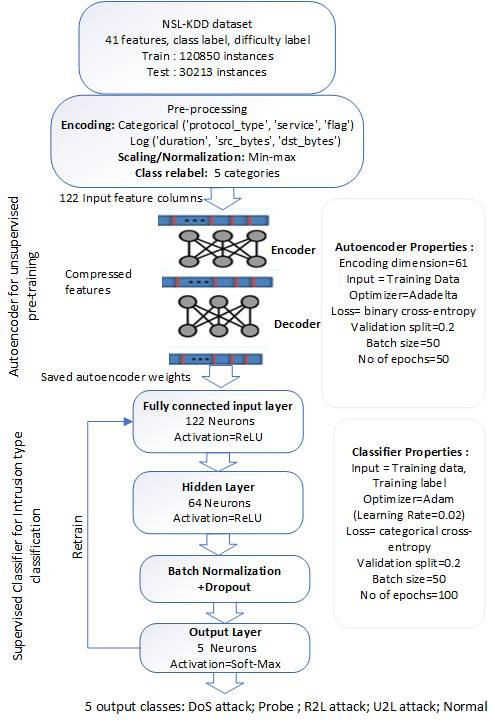
\includegraphics[width=0.89\textwidth]{Figures/NIDS_Autoencoder_Architecture.png}
\caption{Workflow and architecture of the proposed  autoencoded dense neural network}
      \label{fig:Architecture}
    \end{figure}
%
 %\begin{figure}
%      \centering
%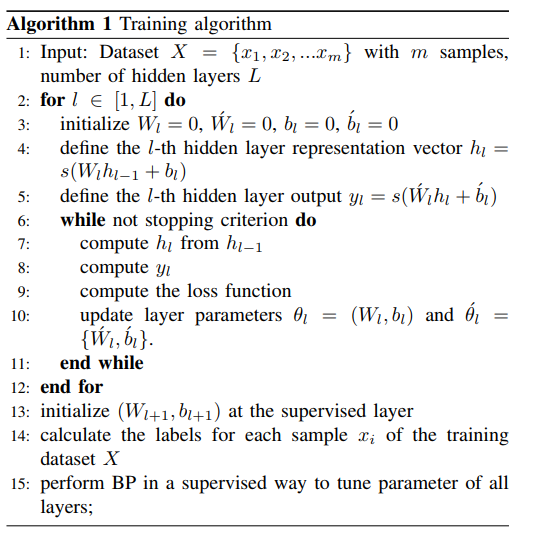
\includegraphics[width=0.49\textwidth]{Figures/Algorithm.PNG}
%\caption{Algorithm}
%\label{fig:Algorithm}
%    \end{figure}



%%%%%%%%%%%%%%%%%%%%%%%%%%%%%%%%%%%%%%%%%%%%%%%%%%%%%%%%%%%%%%%%%%
   
\subsubsection{ Unsupervised pre-training with Autoencoder}
An autoencoder is a type of artificial neural network used to learn efficient data representation in an unsupervised manner. In our proposed model, we have employed an autoencoder with an encoding and a decoding layer  that has been trained to minimize the reconstruction error. This incorporated prior knowledge from the training set to effectively learn from the data itself and provide good performance. Such pre-training allow both the data for the current task and for previous related tasks to self-organize the learning system to build the learning system in a data driven fashion. We have fed the autoencoder with the features from the training dataset without labels (unsupervised). A set of compressed and robust feature is built at the end of this step. The encoder part of the autoencoder aims to compress input data into a low-dimensional
representation, and there is a decoder part that reconstructs input data based on the low-dimension representation generated by the encoder.

For a given training dataset $X = \{x_1, x_2, ..., x_m\}$ with
m samples or instances, where $x_n$ is an n-dimensional feature vector, the
encoder maps the input vector $x_n$ to a hidden representation
vector $h_n$ through a deterministic mapping $f_{\theta}$ as given in \equ{equ:encoder}
\begin{equation}
\label{equ:encoder}
h_n = f_{\theta}(x_n) = \sigma(W x_{n} + b)
\end{equation}
where W is a $p \times p$, p is the number of hidden units, b is a bias vector, $\theta$ is the mapping parameter set $\theta = \{W, b\}$. $\sigma$ is sigmoid activation function.

The decoder maps back the resulting hidden representation
$h_n$ to a reconstructed p-dimensional vector $y_n$ in input space.
\begin{equation}
\label{equ:encoder1}
y_i = g_{\theta}(h_n) = \sigma(W h_{n} + b)
\end{equation}
The goal of training the autoencoder is to minimize the
difference between input and output. Therefore, a error function
is calculated by the following equation:
\begin{equation} E(x,y)= {\frac{1}{m}}\norm{\sum\nolimits_{i=1}^{m}(x_{n}-y_{n})}^{2} \end{equation}
The main objective is to find the optimal parameters to minimize the difference between input and reconstructed output over the whole training set (m).

\subsubsection{ Supervised Classification with DNN}
A three layer dense neural network is employed of a  is trained by using the first auto-encoder,s output as inputs. This task sequence is retrained in a supervised manner with the class labels and the input feature given to the classifier. We have used a softmax activation layer as the output layer. The layer calculates the loss between the predicted values and the true values, and the weights in the network are adjusted according to the loss. 

The simple \emph{softmax} layer, which is placed at the final layer, can be defined as follows:
\begin{align}\label{eq3}
P\left( {c |x} \right) = {\text{argmax}}_{c \in C} \frac{{{ \exp }(x_{L - 1} W_{L} + b_{L} )}}{{\mathop \sum \nolimits_{k = 1}^{{N_{C} }} { \exp }(x_{L - 1} W_{k} )}},
\end{align}
where   $c$  is the number of classes,   $L$  is the last layer index, and $N_{C}$ is the total number of class types including normal network connection and intrusion.
After this stage, all layers are fine-tuned through back-propagation in a supervised way. In the test phase, the softmax layer outputs the probability of the predicted categories. 

%%%%%%%%%%%%%%%%%%%%%%%%%%%%%%%%%%%%%%%%%%%%%%%%%%%%%%%%%%%%%%%%%%

 \begin{figure}
      \centering
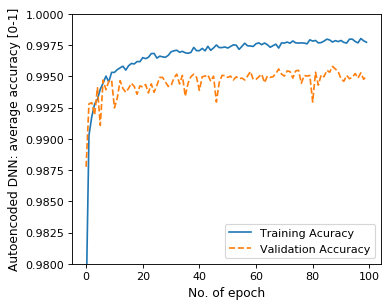
\includegraphics[width=0.7\textwidth]{Figures/Autoencode_DNN.png}
\caption{ Training and validation set accuracy over increasing number of epochs( training iterations) }
      \label{fig:accuracy}
    \end{figure}
%%%%%%%%%%%%%%%%%%%%

\fig{fig:accuracy} plots the performance of the network training process for 100 iterations. During training, we have used additional techniques such as dropout and batch normalization to avoid over fitting and also to speedup the training process. The proposed algorithm   achieves approximately 99\% accuracy for the training set in 20 iterations which is four times faster if no dropout and batch normalization was employed. We used a five-fold cross-validation using 20\% of the training data and the validation data set also achieves high overall accuracy with slight deviation over time. Potentially this allows a reduction in the training epochs required, and will be of vital importance for developing low-latency models and training future networks with bigger data sets.
The proposed algorithm is summarized here in Algorithm I.
%%%%%%%%%%%%%%%%%%%%%%%%%%%%%%%%%%%%%%%%%%%%%%%%%%%%%%%%%%%%%%%%%%%%%


\begin{algorithm}[h]\label{algorithm}
\KwIn{ Taining dataset $X = \{x_1, x_2, ..., x_m\}$, Number of layers $L$}

\nl for $l \in\mathcal [1, L]$ do\;
\nl \ Initialize $ W_l = 0, W´_l = 0, b_l = 0, b'_{l} = 0$\;
 {Encoding layer}\;
\nl \ Calculate encoding or hidden representation using equation(1)\;
\ \  \ \ \  $ h_{l} = s(W_{l}x_{l−1} + b_{l})$\;
{Decoding layer}\;
\nl\ while not loss==stopping criteria do\;
\nl \ \ Compute $y_{l}$ using equation (2)\;
\nl \ \ Compute the loss function: binary cross-entropy\;
\nl\ \ Update layer parameters  $\theta = \{W, b\}$\;
\nl \ end while\;
\nl end for\;
{Classifier:Dense neural network, Soft-max activation at the output layer}\;
\nl Initialize $(W_{l+1}, b_{l+1})$ at the supervised layer\;
\nl {Calculate the labels for each sample $x_n$ of the training dataset $X$}\;
\nl Apply batch normalization and dropout for speeding up the calculation\;
\nl {Perform back-propagation in a supervised manner to tune parameters of all layers, loss function categorical cross-entropy\;}

\nl  end\;
\KwOut{Class labels}
    {\caption{\bf Auto-encoded DNN training algorithm} \label{Algorithm}
    }
\end{algorithm}


\section{Model Evaluation} \label{sec:evaluation}


The main aim of our designed model is to show that the intrusion detection system we designed using deep autoencoded neural network framework will maximize accuracy  and minimize any falsely categorized values.

    \begin{figure*}
      \centering
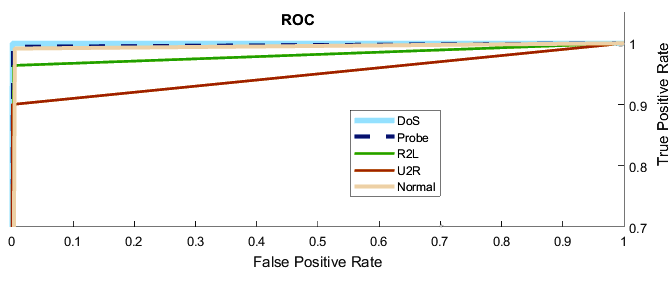
\includegraphics[width=0.89\textwidth]{Figures/ROC.png}
\caption{Receiver operating characteristics for different classes}
      \label{fig:RoC}
    \end{figure*}

\FloatBarrier

\subsection{Model evaluation matrices}
%%%%%%%%%%%%%%%%%% RESULTS %%%%%%%%%%%%%%%%%%

If True Positive ($T_P$) is the number of attacks classified
rightly as attack; True Negative ($T_N$) is the number of normal
events rightly classified normal; False Positive ($F_P$) is the
number of normal events misclassified as attacks and False
Negative ($F_N$) is the number of attacks misclassified as
normal, we can define accuracy, recall, precision and F1 values of a model can be defined using the following equations \cite{SOKOLOVA2009}.

\begin{itemize}
\item {Accuracy: It is an indicator of the total number of correct predictions provided by the model and defined as follows:

\begin{align}
\text{Accuracy} =\frac{T_P+T_N}{T_P+T_N+F_P+F_N}.
\end{align}
}
\item {Recall, precision and F measure: Three of the most commonly used performance measures with F measure being the harmonic mean of recall and precision measures are defined as follows:
\begin{align}
\text{Recall or True positive rate} =\frac{T_P}{T_P+F_N}.
\end{align}
\begin{align}
\text{Precision} =\frac{T_P}{T_P+F_P}.
\end{align}}
\begin{align}
{\text{F \ Measure}} =\frac{2*{\text{Precision}}*{\text{Recall}}}{\text{Precision+Recall}}
\end{align}

 
%\item {F1 Score:It is the harmonic mean of precision and recall and defined as follows:
%\begin{align}
%{\text{F1 \ Score}} =\frac{2*{\text{Precision}}*{\text{Recall}}}{\text{Precision+Recall}}.
%\end{align}}
\end{itemize}
\fig{fig:RoC} showed the class-wise receiver operating characteristic (ROC) for our proposed model. The model produced highly accurate predictions for the classes of the designed NIDS. We obtained a true positive rate (TPR) of above 99\% for normal connection and DoS attack category. The model benefited from comparatively higher number of instances in these two categories. The TPR for the U2R (showed in red in \fig{fig:RoC}) category was 89.2\%, while R2L and Probe attack types had a TPR rate of 94.3\% and 98.4\% respectively. While compared with the ROC curve presented in Shone et al. \cite{Shone2018}, our model achieved much higher TPR values for the under-represented intrusion types R2L and U2R.




\subsection{Confusion Matrix}

We presented the confusion matrix plot  in \fig{fig:confusionmatrix}, for our model when evaluated with the test data set. The rows correspond to the predicted class (Output Class) and the columns correspond to the true class (Target Class).
The diagonal cells in the confusion matrix correspond to observations that are correctly classified ($T_P$ and $T_N$'s). The off-diagonal cells correspond to incorrectly classified observations ($F_P$ and $F_N$'s). Both the number of observations and the percentage of the total number of observations are shown in each cell.
%%%%%%%%%%%%%%%%%%%%%%%%%%%%%%%%%%%%%%%%%%%%%%%%%%%%%%%%%%%%%%%%%%%%%
 \begin{figure}
      \centering
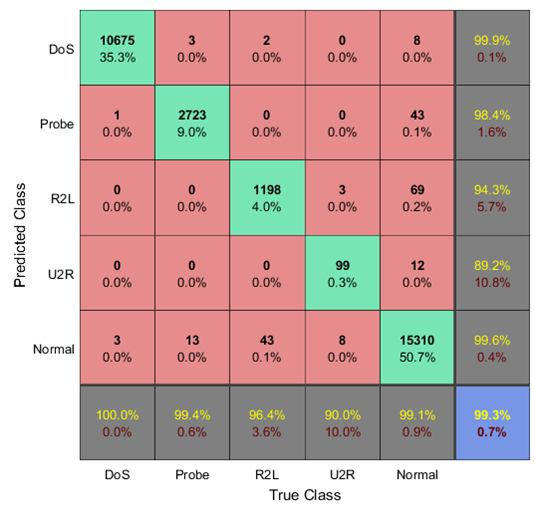
\includegraphics[width=0.75\textwidth]{Figures/Confusion_NIDS.png}
\caption{Confusion matrix of the test dataset}
      \label{fig:confusionmatrix}
    \end{figure}
    

The column on the far right of the plot shows the percentages of all the examples predicted to belong to each class that are correctly and incorrectly classified. These values are often called the precision and false discovery rate respectively. The row at the bottom of the plot shows the percentages of all the examples belonging to each class that are correctly and incorrectly classified. These metrics are often called the recall and false negative rate, respectively. The cell in the bottom right of the plot shows the overall accuracy of the classifier which is 99.3\% in our case. 



To be noted, we have utilized builtin Matlab functions \emph{plotroc(true class, predicted class)} and \emph{plotconfusion(true class, predicted class)} for generating \fig{fig:RoC} and \fig{fig:confusionmatrix}. Both true class and predicted class variables were one-hot encoded and imported from the python interface as .mat file for plotting purposes.

     \begin{table*}
     \centering
    \caption{Quantitative comparison of the proposed method with other deep learning techniques for NSL-KDD 5-class intrusion detection}   \label{table:performance_comparison}
  \begin{tabularx}{\textwidth}{X c c c c c c c}
    \toprule
    Learning method & Year  & DoS (\%) &Probe&R2L&U2R&Normal& Overall Accuracy (\%) \\
    \otoprule
    Self Taught Learning \cite{Javaid2016}&2016&-&-&-&-&-&75.76\\
    Convolutional Neural Networks  \cite{Li2017}& 2017  &-&-&-&-&-& 81.57 \\ 
    
    Deep Belief Network (DBN)  \cite{Shone2018}& 2018 &87.96&72.97 &0&0&95.64  &80.58  \\
   CNN-3 layer\cite{Vinay2017}& 2017 &97.5&92.5&3.43&6.33&99.9& 97.0  \\ 
    CNN 3 layer+LSTM \cite{Vinay2017} & 2017 &99.5&86.8&0.0&7.45&99.7& 98.7 \\ 
   
    \hline
   Deep Neural Network \cite{potluri2016}&2016 &97.7&89.8&13&39.6&95  & 93 \\
    Symmetric Autoencoder(S-NDAE)  \cite{Shone2018}&2018 &94.58&94.67&3.82&2.70 &97.73& 85.42 \\
    Stacked Autoencoder \cite{Farah2018}&2018 &-&-&-&-& - & 94.7 \\
   
    
 \bf{    Proposed Autoencoded DNN} &  2018  &99.9&98.4&94.3&89.2&99.6 &99.3 \\
    \bottomrule
  \end{tabularx}
\end{table*}



\subsection{Comparison with other approaches}

Our results showed an excellent performance with an overall detection accuracy of  99.3\% for Probe, R2L, DoS and U2R type attacks. \tab{table:performance_comparison} summarizes the class-wise true positive rate (TPR) and overall accuracy of our proposed model with some concurrent deep learning methods presented in the literature. All previously reported models in the literature showed poor performance in detecting R2L and U2R type attacks due to lack of data. We up-sampled and restructured the dataset to deal with this discrepancy and the trained model achieved above 89\% accuracy for all the classes. 
   

 
%%%%%%%%%%%%%%%%%% CONCLUSIONS %%%%%%%%%%%%%%%%%%

\section{Conclusions} \label{sec:conclusions}
 Cyber threats have become a prime concern for information security. NIDS is one of the security mechanisms used to guard these applications against attacks. In this research, we have applied a deep network intrusion detection model and evaluated the algorithm with the benchmark NSL-KDD dataset. Currently, the algorithm is trained offline on high performance computer. Our  results  showed  an  excellent  performance  with  an overall  detection  accuracy  of  99.3\%  for  Probe,  R2L,  DoS and  U2R type  of attacks. We also presented a comparison with recent approches used in literature which showed a substantial improvement in terms of accuracy and latency with proposed autoencoded DNN. In future, we will provide extensions or modifications of the proposed algorithm for mobile and IoT security platforms as suggested in ref \cite{ABAWAJY2018} using intelligent agents  such as soft computing and advanced unsupervised clustering algorithms. Because of the availability of deep learning libraries in python such as Keras and TensorFlow Lite \cite{tensorflowlite}, on-device machine learning inference is now possible with low latency. Hence, future models will cover a broader range of attacks, respond in real time and update itself over time. Future extension of this work will be to improve the detection accuracy and to reduce the rate of false negative and false positive rate in attack detection to improve the systems performance. In future, we will also continue our efforts for improvements to the approach and will apply the technique on similar but more recent and complex datasets such as Aegean  Wi-Fi  Intrusion  Dataset  (AWID) \cite{AWID}, UNSW-NB15dataset \cite{UNSW-dataset2015}.
 \FloatBarrier

%%%%%%%%%%%%%%%%%% REFERENCES %%%%%%%%%%%%%%%%%%
\renewcommand*{\bibfont}{\small}
\printbibliography

\end{document}
